% Fig. 1: from a conversion of the free-running delta-sigma ADC to the UTC time of its sample.
% Two-column figure (at most 7.16 in wide). Built by `make figures` into figures/out/timing_chain.pdf.
\documentclass[tikz,border=1pt]{standalone}
\usepackage[T1]{fontenc}
\usepackage{newtxtext,newtxmath}
\usepackage{siunitx}
\usetikzlibrary{positioning,arrows.meta,calc}
\definecolor{okblue}{HTML}{0072B2}
\definecolor{okgray}{HTML}{7F7F7F}
\sisetup{range-phrase={--}, range-units=single}

\begin{document}
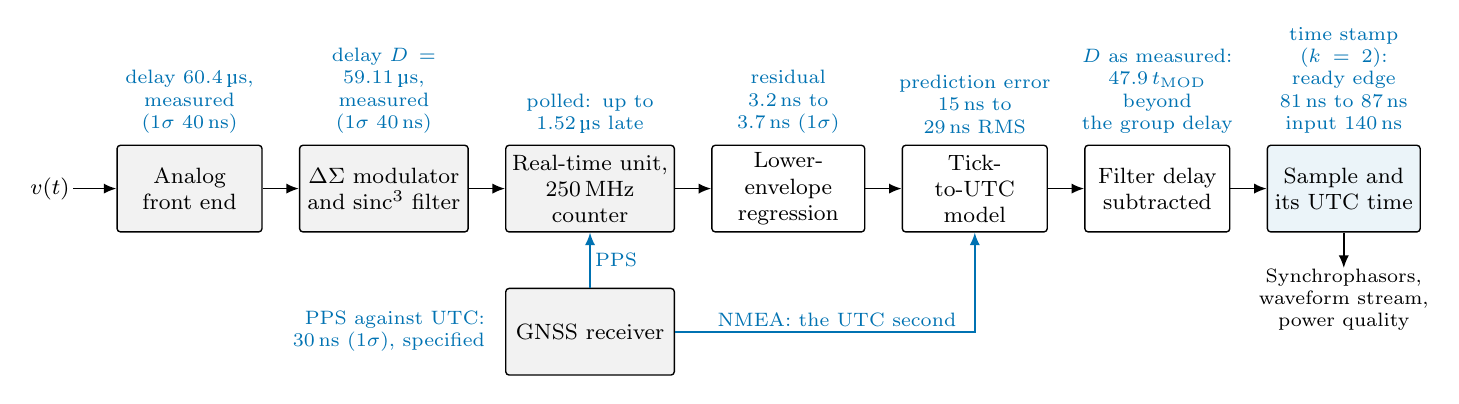
\begin{tikzpicture}[
    font=\footnotesize,
    node distance=4.6mm,
    box/.style={draw, line width=0.5pt, rounded corners=1.2pt, align=center, inner sep=2pt,
                minimum height=11mm, text width=#1},
    box/.default=19mm,
    hw/.style={box=#1, fill=black!5},
    hw/.default=19mm,
    signal/.style={-{Latex[length=1.6mm,width=1.3mm]}, line width=0.6pt},
    time/.style={-{Latex[length=1.6mm,width=1.3mm]}, line width=0.6pt, okblue},
    note/.style={font=\scriptsize, okblue, align=center, inner sep=0pt, text width=#1, anchor=south},
    note/.default=21mm,
  ]
  % Signal path: hardware (shaded), then software
  \node[hw=17mm] (front) {Analog\\front end};
  \node[hw=20mm, right=of front] (adc) {$\Delta\Sigma$ modulator\\and sinc$^3$ filter};
  \node[hw=20mm, right=of adc] (pru) {Real-time unit,\\\SI{250}{\mega\hertz} counter};
  \node[box=18mm, right=of pru] (env) {Lower-envelope\\regression};
  \node[box=17mm, right=of env] (utc) {Tick-to-UTC\\model};
  \node[box=17mm, right=of utc] (delay) {Filter delay\\subtracted};
  \node[box=18mm, right=of delay, fill=okblue!8] (out) {Sample and\\its UTC time};

  \draw[signal] ($(front.west)+(-5.5mm,0)$) node[left, inner sep=1pt] {$v(t)$} -- (front);
  \foreach \a/\b in {front/adc, adc/pru, pru/env, env/utc, utc/delay, delay/out}
    \draw[signal] (\a) -- (\b);

  % What each stage leaves in the time, on one line above the boxes
  \coordinate (top) at ($(front.north)+(0,1.4mm)$);
  \node[note=19mm] at (front.north |- top) {delay \SI{60.4}{\micro\second},\\measured ($1\sigma$ \SI{40}{\nano\second})};
  \node[note] at (adc.north |- top) {delay $D=\SI{59.11}{\micro\second}$,\\measured ($1\sigma$ \SI{40}{\nano\second})};
  \node[note] at (pru.north |- top) {polled: up to\\\SI{1.52}{\micro\second} late};
  \node[note] at (env.north |- top) {residual\\\SIrange{3.2}{3.7}{\nano\second} ($1\sigma$)};
  \node[note] at (utc.north |- top) {prediction error\\\SIrange{15}{29}{\nano\second} RMS};
  \node[note] at (delay.north |- top) {$D$ as measured:\\$47.9\,t_\mathrm{MOD}$ beyond\\the group delay};
  \node[note] at (out.north |- top) {time stamp ($k=2$):\\ready edge \SIrange{81}{87}{\nano\second}\\input \SI{140}{\nano\second}};

  % Time path
  \node[hw=20mm, below=7mm of pru] (gnss) {GNSS receiver};
  \draw[time] (gnss.north) -- node[right, font=\scriptsize, inner sep=1.5pt] {PPS} (pru.south);
  \node[font=\scriptsize, okblue, align=right, anchor=east, inner sep=0pt] at ($(gnss.west)+(-2.5mm,0)$)
    {PPS against UTC:\\\SI{30}{\nano\second} ($1\sigma$), specified};
  \draw[time] (gnss.east) -| node[pos=0.27, above, font=\scriptsize, inner sep=1.5pt] {NMEA: the UTC second} (utc.south);

  % Its users
  \node[below=4.5mm of out, align=center, font=\scriptsize, text width=22mm, inner sep=0pt] (uses)
    {Synchrophasors,\\waveform stream,\\power quality};
  \draw[signal] (out.south) -- (uses.north);
\end{tikzpicture}
\end{document}
